\documentclass{webofc}
\usepackage[varg]{txfonts}
\usepackage{xspace}
\usepackage{hyperref}

\newcommand{\tauo}{\ensuremath{c\tau_{0}}\xspace}
\newcommand{\ctau}{\ensuremath{c\tau_{0}}\xspace}
\newcommand{\gluino}{\ensuremath{\tilde{\textrm{g}}}\xspace}
\newcommand{\lsp}{\ensuremath{\tilde{\chi}_{1}^{0}}\xspace}
\newcommand{\pt}{\ensuremath{p_\textrm{T}}\xspace}
\newcommand{\jht}{\ensuremath{H_\textrm{T}}\xspace}
\newcommand{\jmht}{\ensuremath{H_\textrm{T}^\textrm{miss}}\xspace}
\newcommand{\met}{\ensuremath{p_\textrm{T}^\textrm{miss}}\xspace}
\newcommand{\ttbar}{\ensuremath{\textrm{t}\bar{\textrm{t}}}\xspace}
\newcommand{\wjets}{\ensuremath{\textrm{W+jets}}\xspace}
\newcommand{\znunu}{\ensuremath{\textrm{Z}(\to\nu\bar{\nu})\textrm{+jets}}\xspace}
\begin{document}

\title{Identification of new long-lived particles using deep neural networks}

\author{\firstname{Matthias} \lastname{Komm} \inst{1}\fnsep\thanks{\email{Matthias.Komm@cern.ch}}, for the CMS Collaboration}

\institute{CERN, Geneva, Switzerland}

\abstract{
We present the development of a deep neural network for identifying generic displaced jets arising from the decays of exotic long-lived particles in data recorded by the CMS detector at the CERN LHC. Various jet features including detailed information about each clustered particle candidate as well as reconstructed secondary vertices are refined through the use of 1-dimensional convolution layers before being combined with high-level engineered features and passed through a series of fully-connected layers. The proper lifetime of the long-lived particle, \tauo, is treated as a parameter of the neural network model, which allows for hypothesis testing over several orders of magnitude ranging from $\ctau = 1\,\mu\textrm{m}$ to 10\,m. Domain adaptation by backward propagation is performed to construct domain-independent features at an intermediate layer of the network to mitiage difference between simulation and data. The training is performed by streaming ROOT trees containing $\mathcal{O}$(100M) jets directly into the TensorFlow queue system, which allows for a flexible selection of input features and asynchronous preprocessing. The application of the tagger is showcased in a search for long-lived gluinos as predicted by split supersymmetric models demonstrating significant gains in sensitivity over a reference analysis.
}

\maketitle

\section{Introduction}
\label{intro}

Machine-learned algorithms are routinely deployed to perform event reconstruction, particle identification, event classification, and other tasks~\cite{ml-white-paper} when analysing data samples recorded by experiments at the CERN LHC. For example, the ATLAS~\cite{atlas} and CMS~\cite{cms} Collaborations have developed numerous algorithms based on boosted decision trees or neural networks to identify jets originating from the hadronisation of bottom quarks with unprecedented performance~\cite{batlas,bcms}.

This note, based on Ref.~\cite{CMS-EXO-19-011}, summarises the development and application of a novel algorithm for identifying jets originating from the decay of long-lived particles (LLPs). The algorithm is based on a deep neural network (DNN) that is inspired by the CMS DeepJet approach~\cite{dj}, albeit several aspects required an extension of the DeepJet architecture and training procedure. To perform supervised learning a generic definition for displaced jets is introduced. Furthermore, the DNN is parametrised as a function of the proper lifetime, \tauo, of the long-lived particle to allow hypothesis testing over several orders of magnitude ranging from $\ctau = 1\,\mu\textrm{m}$ to 10\,m. To mitigate uncertainties arising from difference between simulation and data, domain adaptation by backward propagation~\cite{da} is applied during the training. The application of the resulting DNN is demonstrated in a search for long-lived gluino production as predicted by split supersymmetric (SUSY) models~\cite{splitsusy}.

\section{Simulated samples and jet labelling}
\label{samples}

The DNN is trained on labelled anti-$k_t$ jets with $\pt>20~\mathrm{Gev}$ and $|\eta|<2.4$ that are clustered from candidates reconstructed with the particle-flow (PF) algorithm~\cite{pf} using a distance parameter of 0.4. Jets from the hadronisation of gluons, light-flavoured quarks (uds), and charm or bottom quarks are used as background classes in the DNN training. These are taken from simulated samples of multijet events produced via the strong interaction, a manifestation of quantum chromodynamics (QCD), and top quark pair production. Signal jets from LLP decays are taken from various samples of simulated split SUSY events containing pair-produced long-lived gluinos (\gluino) that decay into a light quark/antiquark pair and a neutralino (\lsp) with varying lifetime and gluino/neutralino masses. At the LLP decay vertex, the two quarks can still interact which each other resulting often in more than only two distinct jets as shown in Fig.~\ref{decay} for two example gluino decays.

\begin{figure*}[!ht]
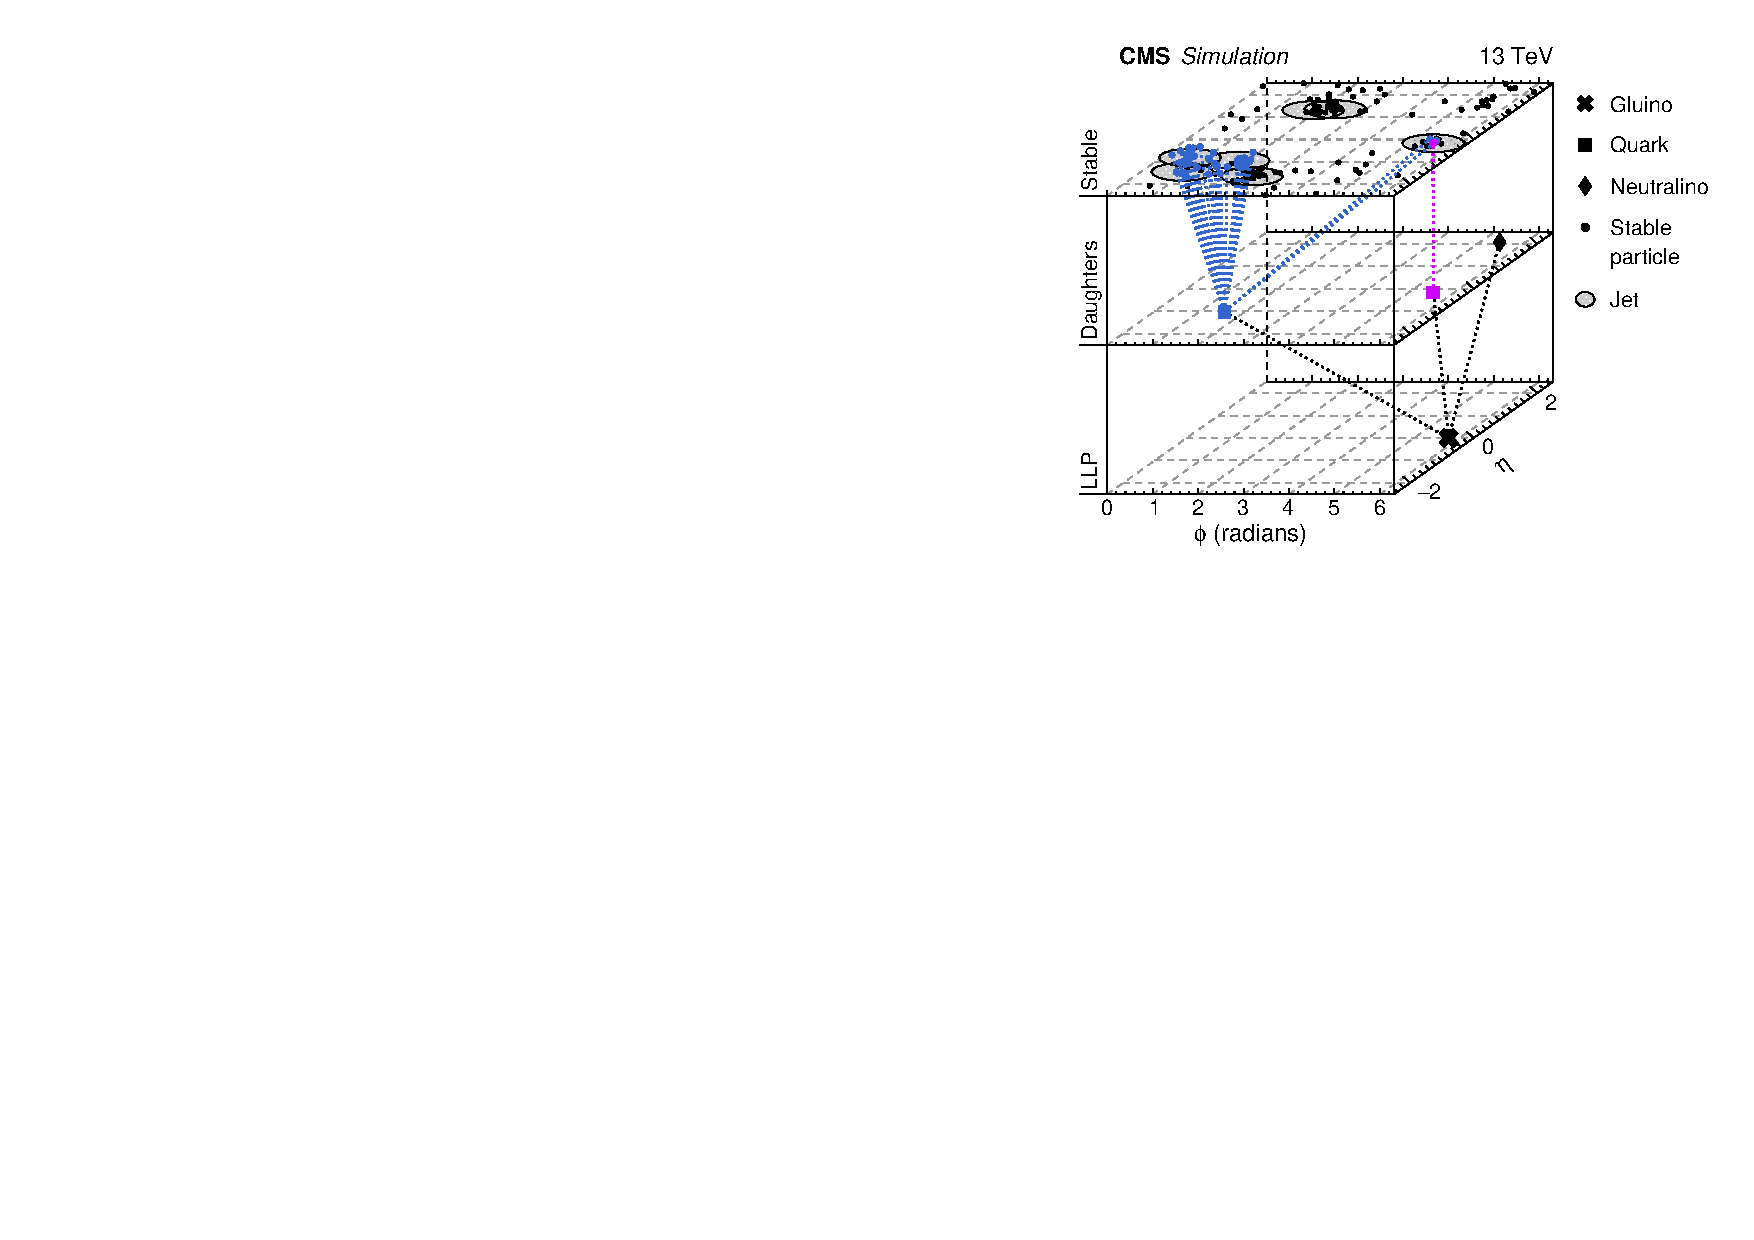
\includegraphics[width=0.48\textwidth]{figs/decay1.pdf}\hspace{0.03\textwidth}
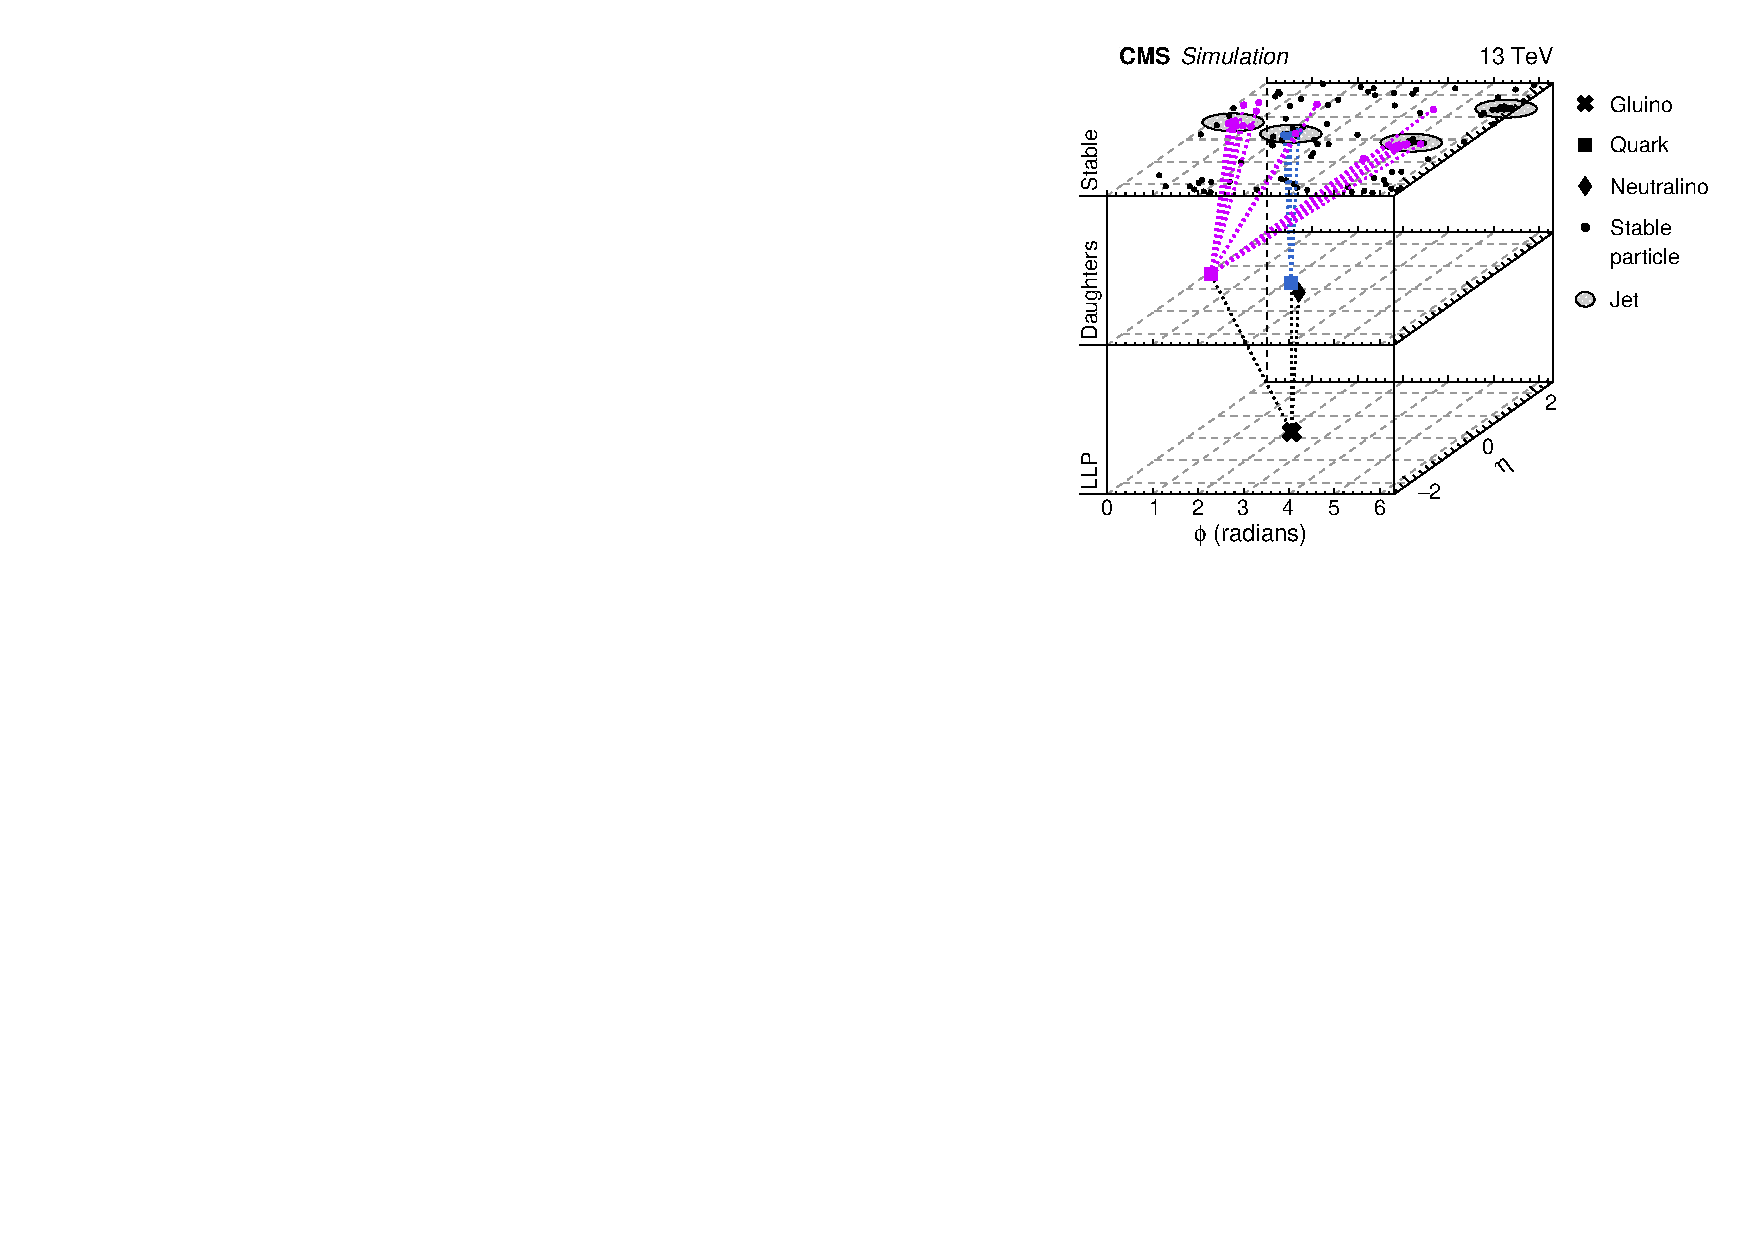
\includegraphics[width=0.48\textwidth]{figs/decay2.pdf}
\centering
\caption{Two example decays of a gluino into a quark/antiquark pair and a neutralino. The positions in $\eta$ and $\phi$ of the gluino, the quarks and neutralino, and the jets clustered from the stable particles after hadronisation are shown in the lower, middle, and top layer, respectively. The figures are taken from Ref.~\cite{CMS-EXO-19-011}.}
\label{decay}
\end{figure*}

A novel definition of a generic LLP jet is introduced by labelling only those jets as 'LLP' for which most of the momentum is carried by clustered particles stemming from the gluino decay vertex, determined from generator-truth information.


\section{Deep neural network architecture and training}
\label{dnn}

An overview of the DNN architecture is given in Fig.~\ref{arch}. In total, approximately 600 input features are considered. The features associated with the clustered charged and neutral jet constituents and the secondary vertices are compressed through a series of one-dimensional convolutions with a kernel size of one. These are then combined with the LLP lifetime and global jet features. After a single dense layer with 200 nodes the network is split in two parts. The top part attempts to predict the jet label, whereas the bottom part predicts the domain of a jet, i.e. if a jet stems from data or simulation. Domain adaptation by backward propagation~\cite{da} is performed by reversing the gradients of the domain loss with respect to the network weights in the preceding layers as indicated. When minimising the combined loss $L_\mathrm{class}+\lambda\,L_\mathrm{domain}$, the network is forced to only retain features that are domain-invariant. The strength of this effect is controlled through the hyperparameter $\lambda$.

\begin{figure*}[!ht]
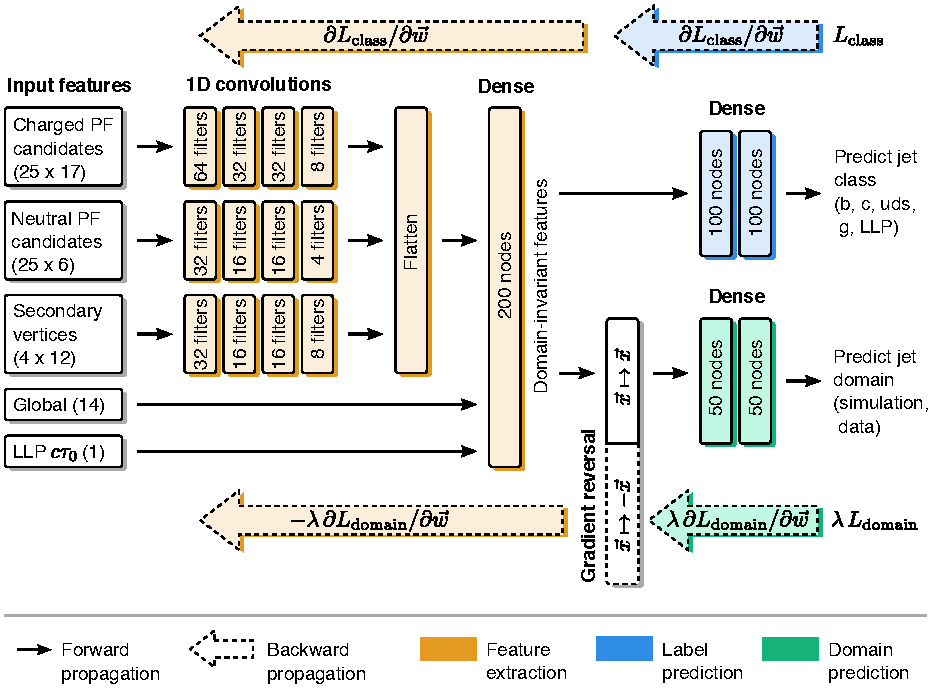
\includegraphics[width=0.9\textwidth]{figs/network.pdf}
\centering
\caption{An overview of the DNN architecture, which comprises convolutional and dense layers; the numbers of filters and nodes are indicated. The input features are grouped by object type and ($m\times n$) indicates the maximum number of objects ($m$) and the number of features per object ($n$). The gradients of the class ($L_\textrm{class}$) and domain ($L_\textrm{domain}$) losses with respect to the weights $w$, used during backward propagation, are shown. The figure is taken from Ref.~\cite{CMS-EXO-19-011}.}
\label{arch}
\end{figure*}

Data from a control region consisting of events with at least two jets and exactly one isolated muon is used in the DNN training for domain adaptation. The resulting agreement between data and simulation is validated in an independent control region in which events are required to contain at least two jets and exactly two isolated muons instead. The distribution of the maximum LLP likelihood predicted by the network over all selected jets within an event is shown in Fig.~\ref{da}. Applying domain adaptation results in a good agreement with negligible uncertainties remaining, whereas deviations of up to 50\% appear in the binned counts between data and simulation when training the DNN without domain adaptation.

\begin{figure*}[!ht]
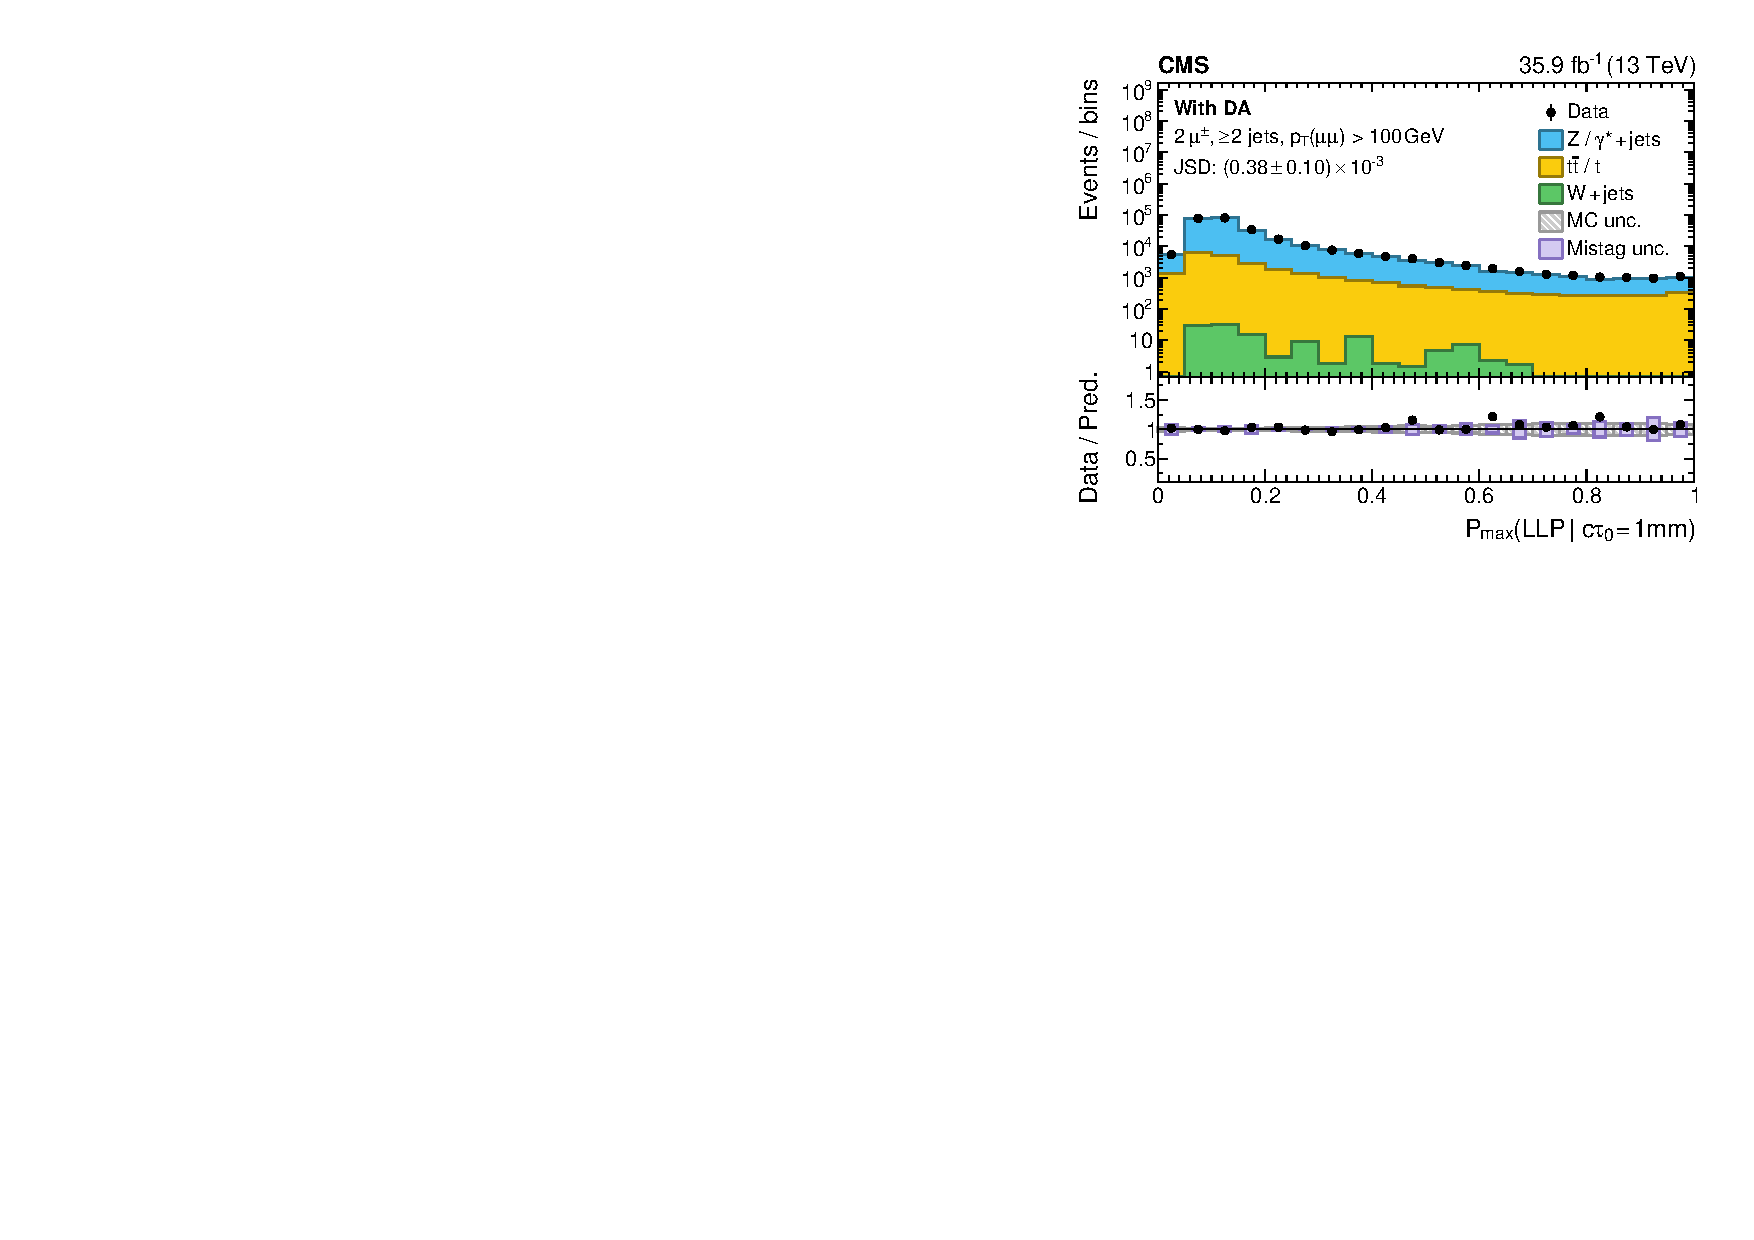
\includegraphics[width=0.48\textwidth]{figs/2mu_2toNj__llpdnnx_da_0_max_highpt.pdf}\hspace{0.03\textwidth}
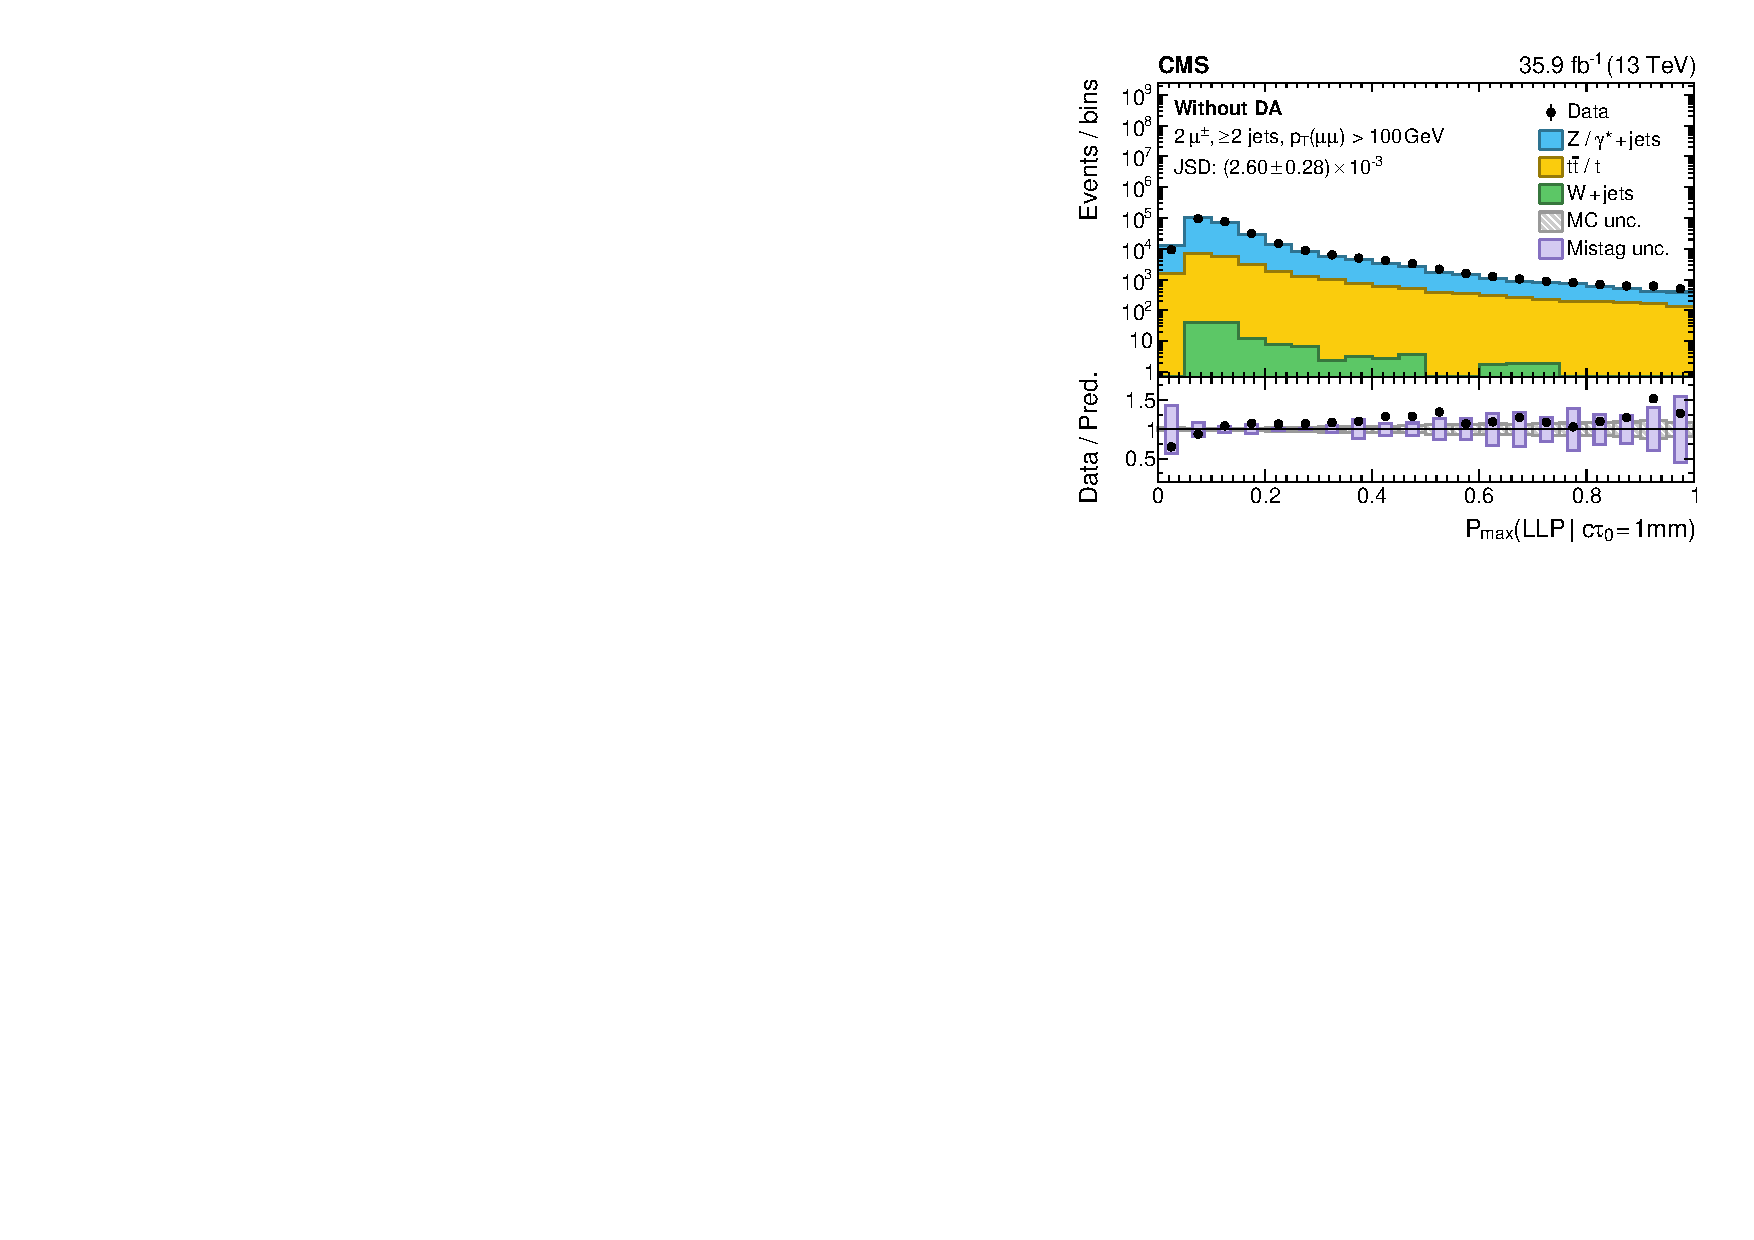
\includegraphics[width=0.48\textwidth]{figs/2mu_2toNj__llpdnnx_noda_0_max_highpt.pdf}
\centering
\caption{Distributions of the maximum probability of the LLP jet class per event in a control region consisting of two isolated muons and at least two jets with (left) and without (right) domain adaptation applied. The figures are taken from Ref.~\cite{CMS-EXO-19-011}.}
\label{da}
\end{figure*}

To train the DNN efficiently on a large sample of jets ($\mathcal{O}$(100M)), taken from data and simulation, a novel interface between ROOT TTrees and TensorFlow/Keras has been developed in the context of this work. Custom operational kernels are used to read jets from ROOT TTrees and produce corresponding tensors that are preprocessed and streamed into the Tensorflow queue system asynchronously and in parallel to the training cycle. The preprocessing encompasses a resampling of jets such that similar distributions in $(\pt,\eta)$ is achieved for all classes. Furthermore, random \ctau values are drawn from the distribution of LLP jets and assigned to non-LLP jets per batch on-the-fly. A demonstration of the workflow can be found in Ref.~\cite{code}.

\section{Performance}
\label{peformance}

The performance of the resulting classifier is assessed by comparing the LLP jet selection efficiency against the rate of rejecting udsg jets as found in an inclusive \ttbar sample. The LLP jet classification efficiency for a fixed misidentification rate of 0.01\% is shown in Fig.~\ref{fig:roc} on the left as a function of the gluino lifetime for two example split SUSY scenarios. The tagger is able to identify LLP jets with efficiencies of about 40--80\% over various orders of \ctau ranging from 1\,\textrm{mm} to 10\,\textrm{m}. The LLP efficiency as a function of the misidentification rate for LLP jets from split SUSY or from two alternative LLP models, gauge-mediated SUSY breaking (GMSB)~\cite{gmsb} resulting in displaced gluon jets and weak $R$-party violation (RPV)~\cite{rpv} resulting in displaced b jets, is presented in Fig.~\ref{fig:roc} on the right, where the latter two have not been used in the training. Comparable performance is seen within uncertainties for all three models, which demonstrates good generalisation of the tagger and furthermore shows that the LLP identification efficiency depends little on the jet flavour.

\begin{figure*}[!ht]
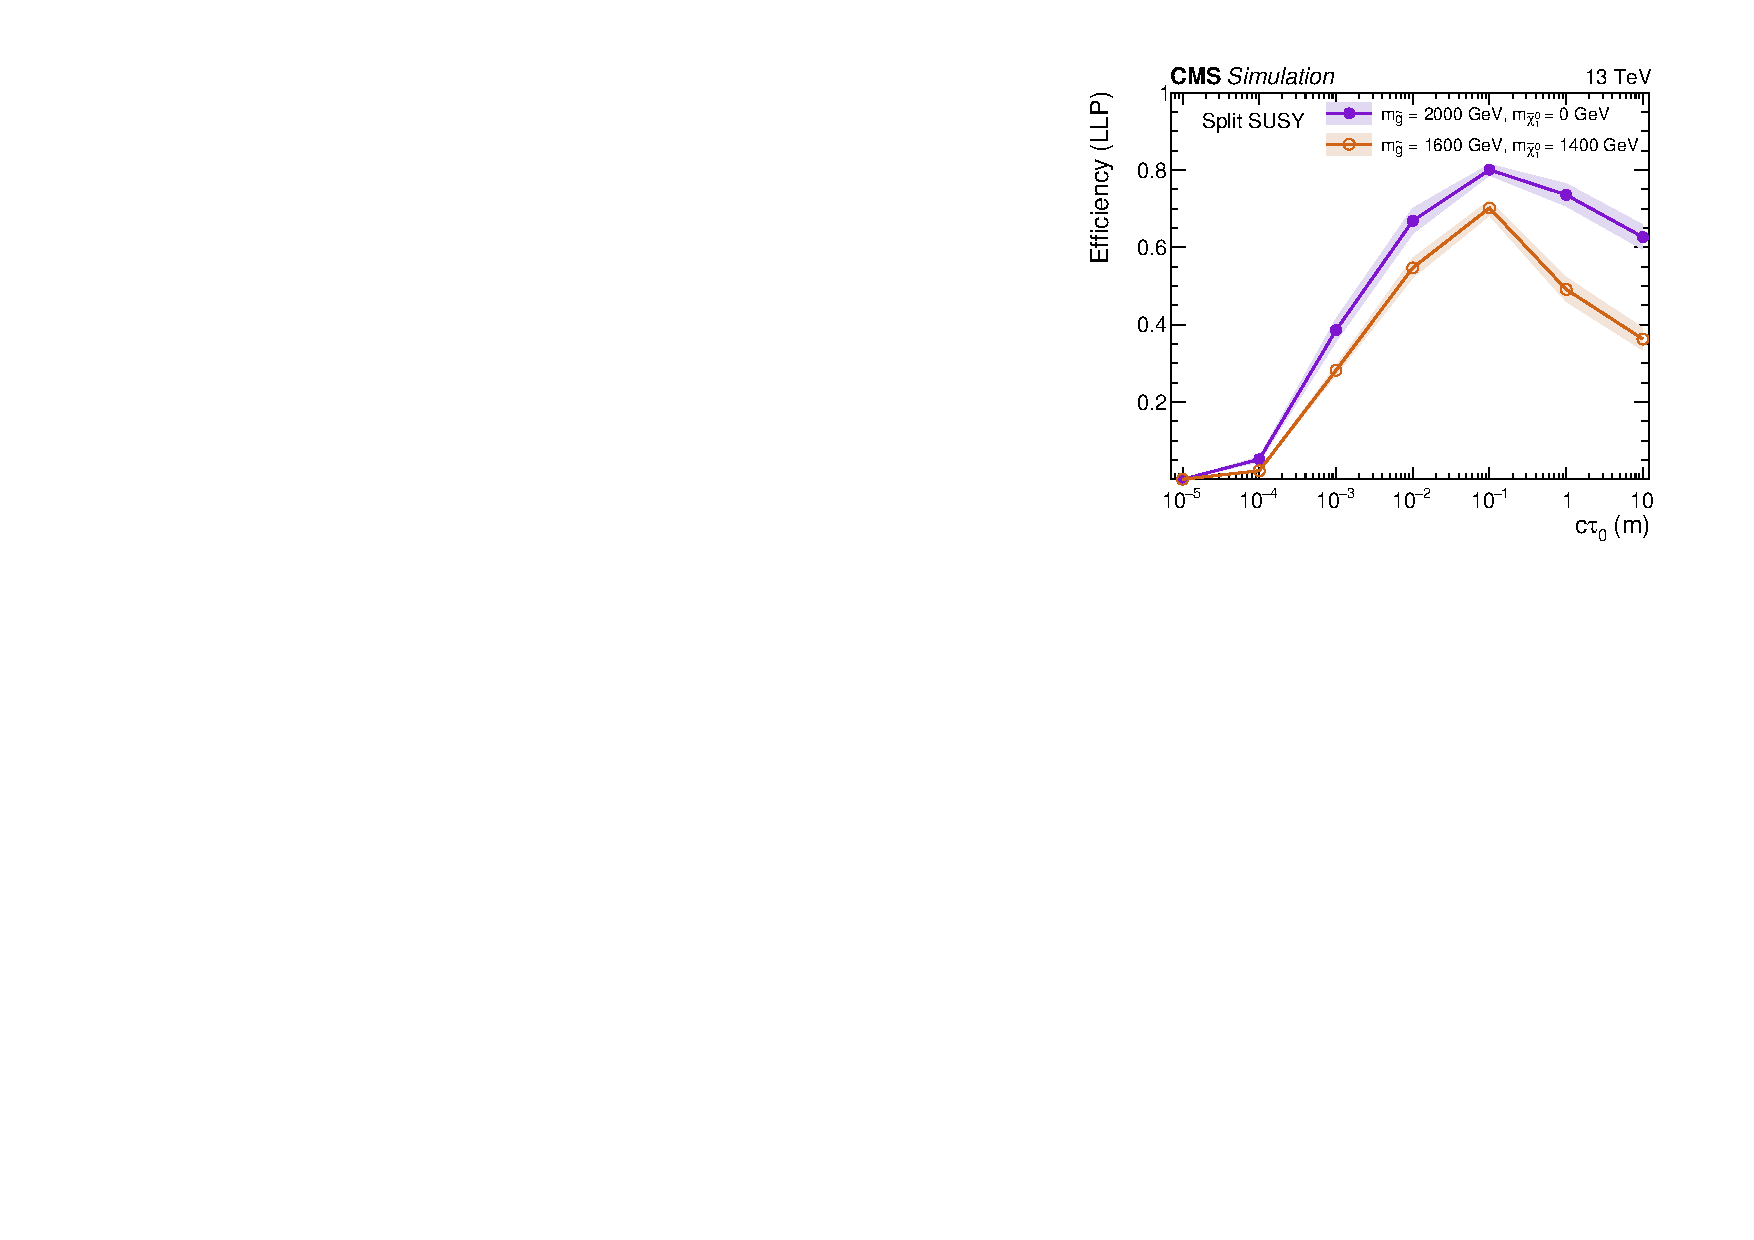
\includegraphics[width=0.48\textwidth]{figs/ctau.pdf}\hspace{0.03\textwidth}
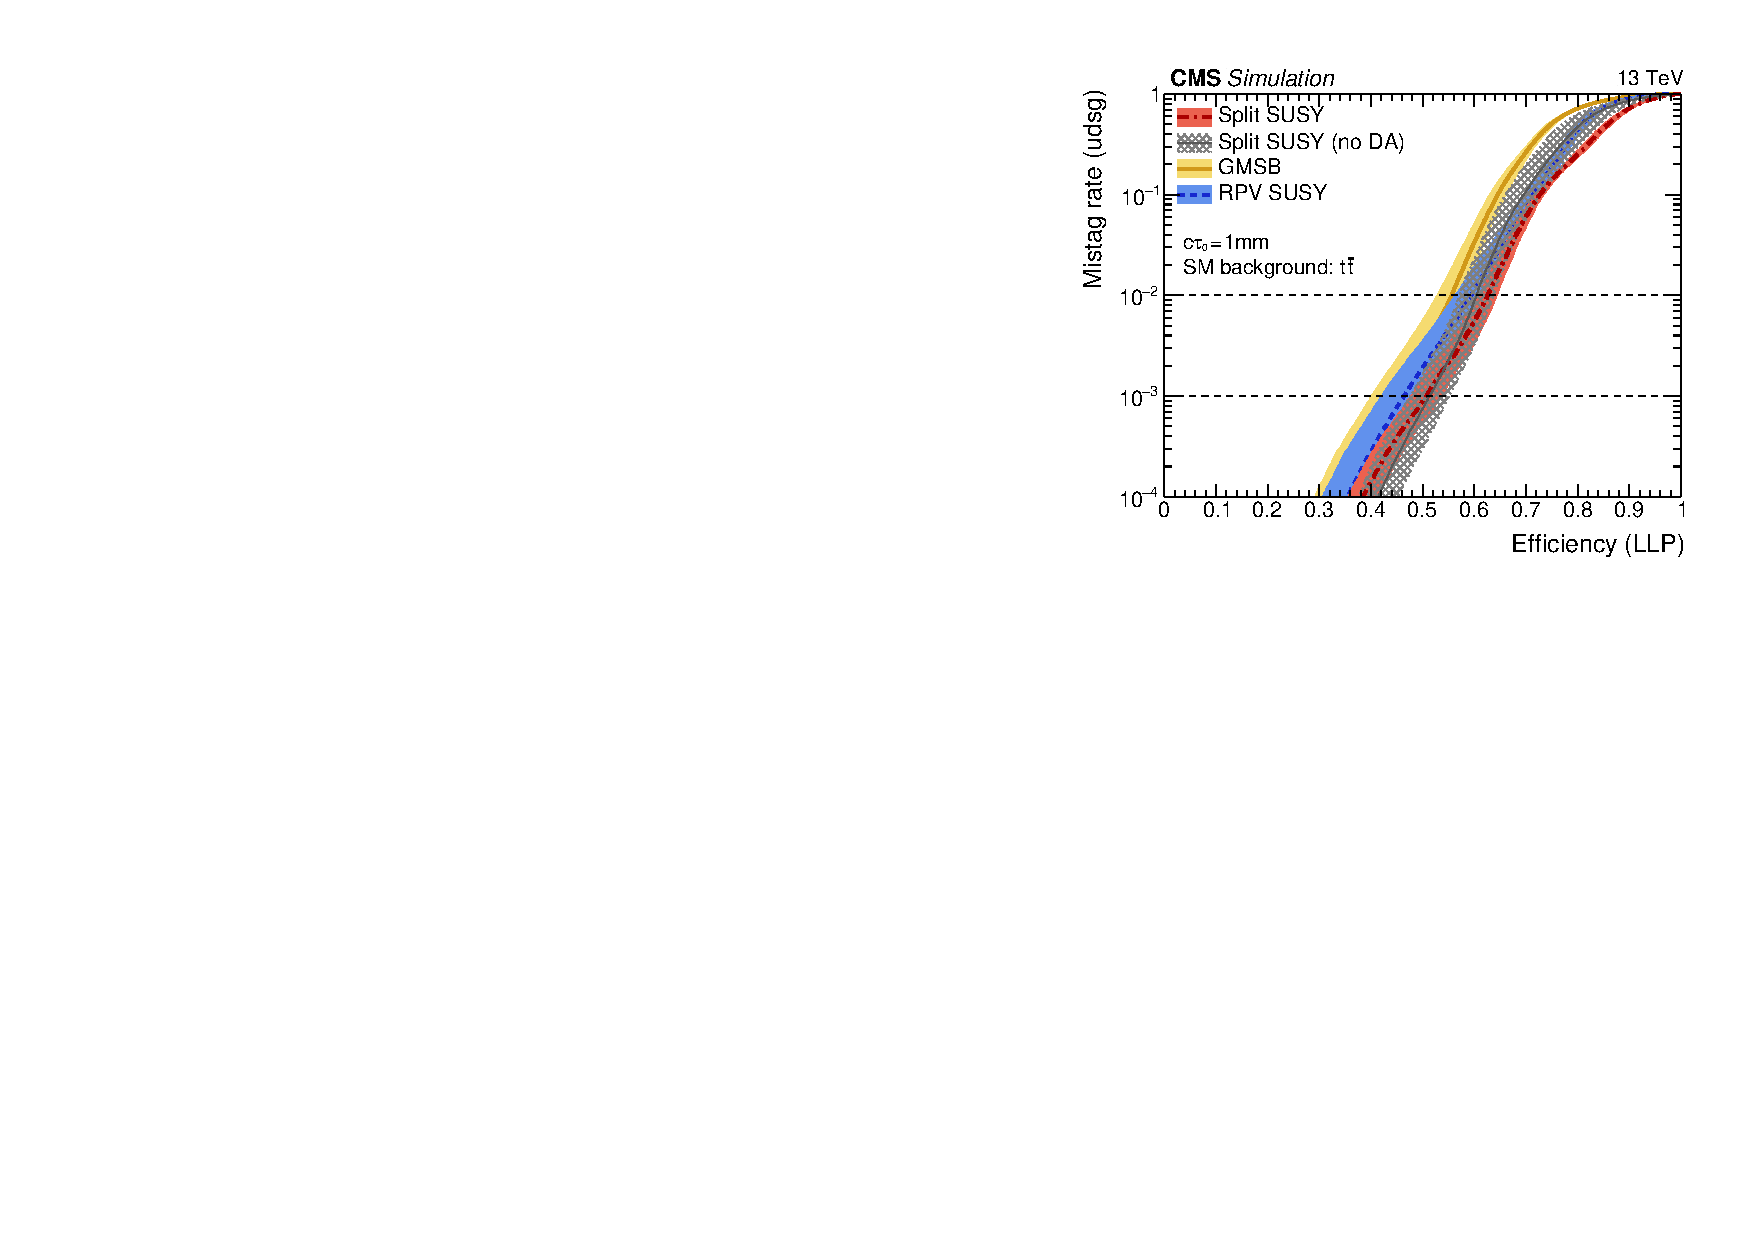
\includegraphics[width=0.48\textwidth]{figs/roc_1.pdf}
\centering
\caption{\label{fig:roc}Performance of identifying LLP jets while rejecting udsg jets from an inclusive \ttbar sample: (left)~LLP jet selection efficiency for a fixed background rate of 0.01\% as a function of \ctau; (right)~the receiver operator characteristic (ROC) curves for three different LLP models with $\ctau=1\,\textrm{mm}$. The figures are taken from Ref.~\cite{CMS-EXO-19-011}.}
\label{fig-3}
\end{figure*}

\section{Showcase search for long-lived gluinos}
\label{showcase}

In the following, the application of the tagger is demonstrated in a search for long-lived gluinos as predicted in split SUSY with $10\,\mu\textrm{m}<\ctau<10\,\textrm{m}$. Expected limits on the theoretical gluino pair production cross section are determined, while assuming the conditions of the recorded proton-proton collision data set in 2016 at $\sqrt{s}=13\,\textrm{TeV}$ by the CMS experiment that corresponds to $35.9\,\textrm{fb}^{-1}$.

Signal events are required to contain at least three jets with $\pt>30\,\textrm{GeV}$ and $|\eta|<2.4$ and no isolated muons (electrons) with $\pt>10(15)\,\textrm{GeV}$ within $|\eta|<2.4$ that also pass loose identification criteria. Furthermore, the scalar and vectorial \pt sum of jets, $\jht=\sum_{i}^\textrm{jets}\pt^{i}$ and $\jmht=|\sum_{i}^\textrm{jets}\vec{p}_\textrm{T}^{i}|$, are required to be both larger than $300\,\textrm{GeV}$. Multijet events are suppressed to a negligible level by requiring $\jmht/\met<1.25$ and that the minimum azimuthal separation between each jet and the $\jht$ of all other jets is greater than 0.2 radians. The remaining events are categorised according to the number of jets, the number of jets that also pass a predefined LLP probability threshold, and \jht. The largest remaining background processes are found to be \wjets, \znunu, single top quark, and \ttbar production. 

The signal and background yields in each category are affected by several sources of systematic uncertainties. This encompasses uncertainties in the background normalisations, the jet energy scale and resolution, the energy scale of the unclustered component of \met, the number of pileup interactions, the renormalisation and factorisation scales, the misidentification of background jets as LLP jets, and the luminosity. The unknown LLP jet identification efficiency in data is estimated in-situ by including an additional nuisance parameter in the likelihood that modifies the scale and shape of the signal template taken from simulation depending on the number of tagged and untagged true LLP jets per category.

Expected 95\% CL upper limits on the gluino mass as a function of \ctau for two example scenarios are shown in Fig.~\ref{fig:limits}. The results are compared to an inclusive search for SUSY~\cite{refsearch} that has been performed on the same data set. The usage of the developed LLP tagger allows to excluded significantly larger gluino masses of up to $500\,\textrm{GeV}$ for $\ctau\gtrsim1\,\textrm{mm}$. The results are also found competitive with respect to a dedicated search with an optimised reconstruction technique~\cite{atlasref}.
 
\begin{figure*}[!ht]
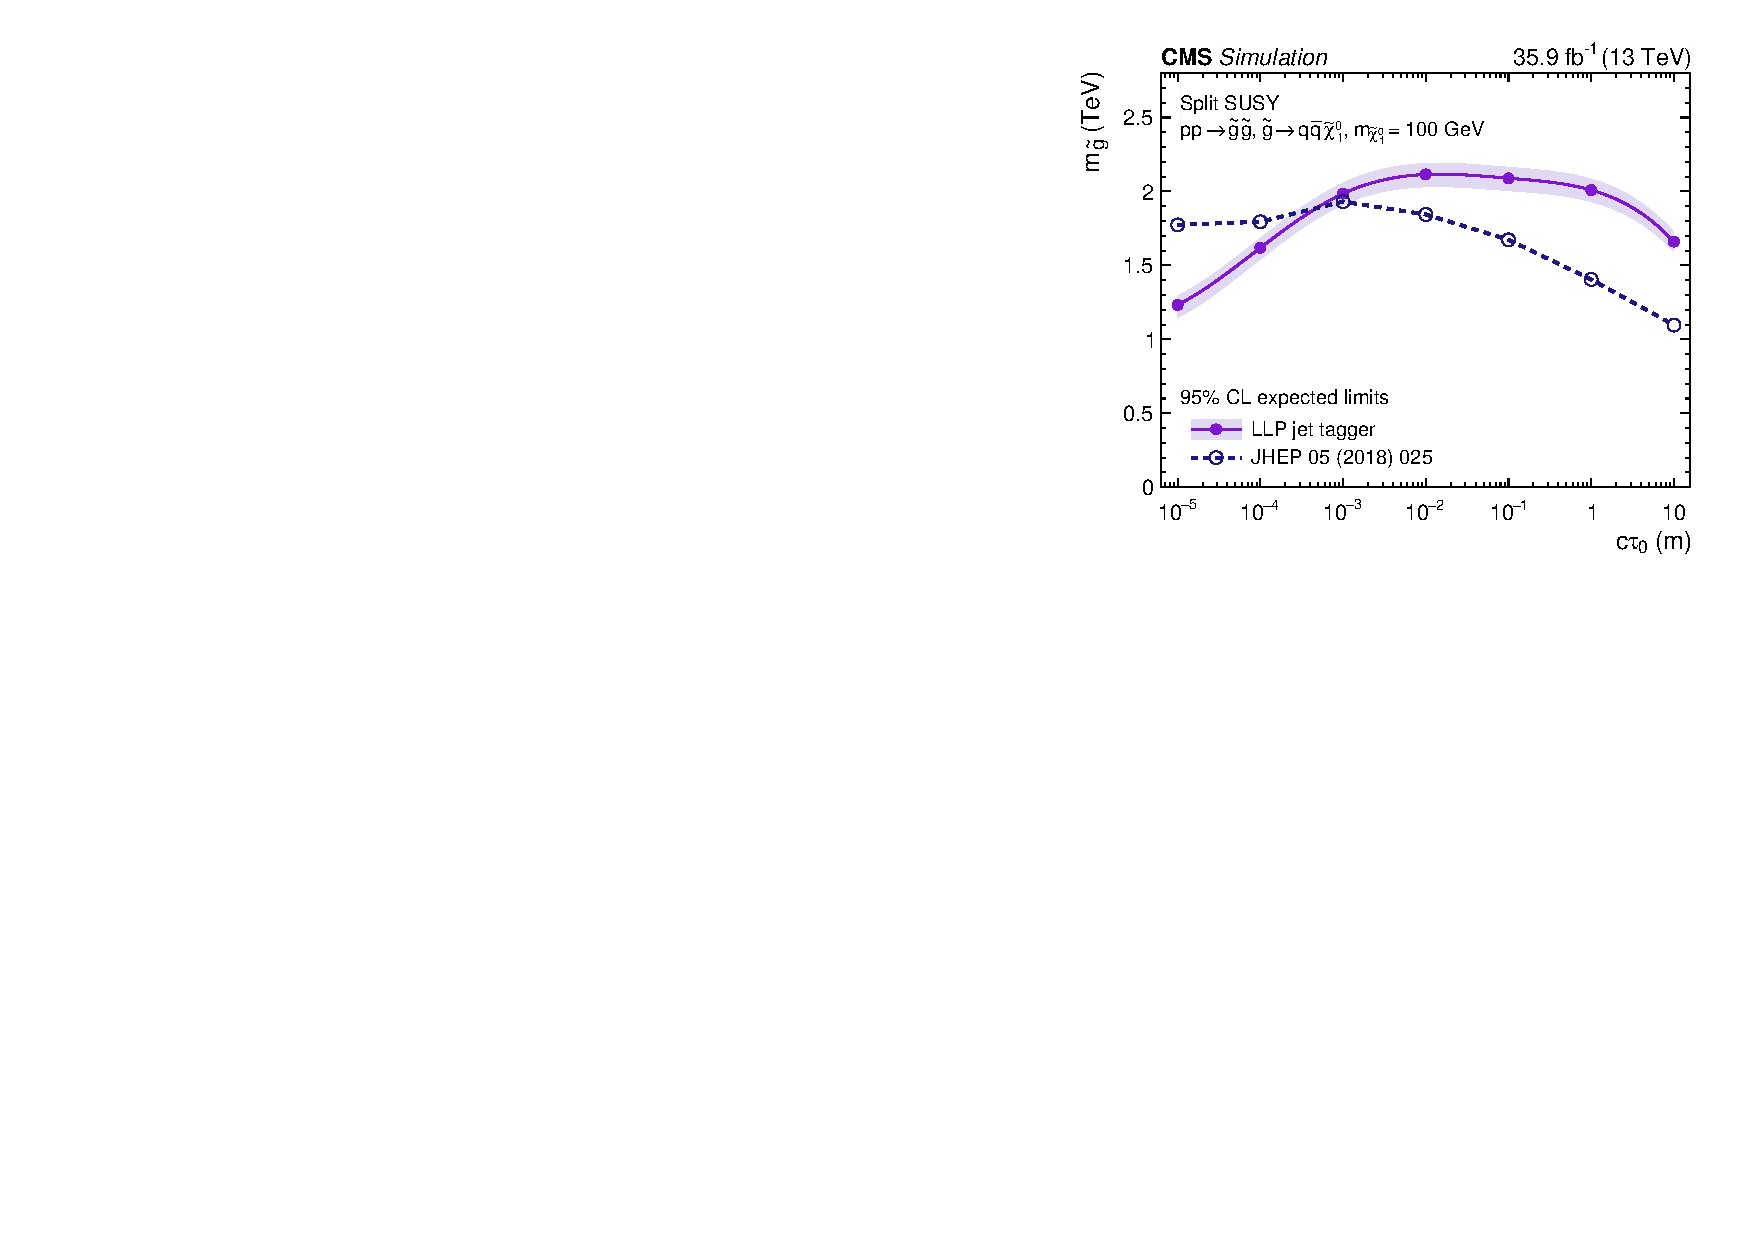
\includegraphics[width=0.48\textwidth]{figs/summaryU.pdf}\hspace{0.03\textwidth}
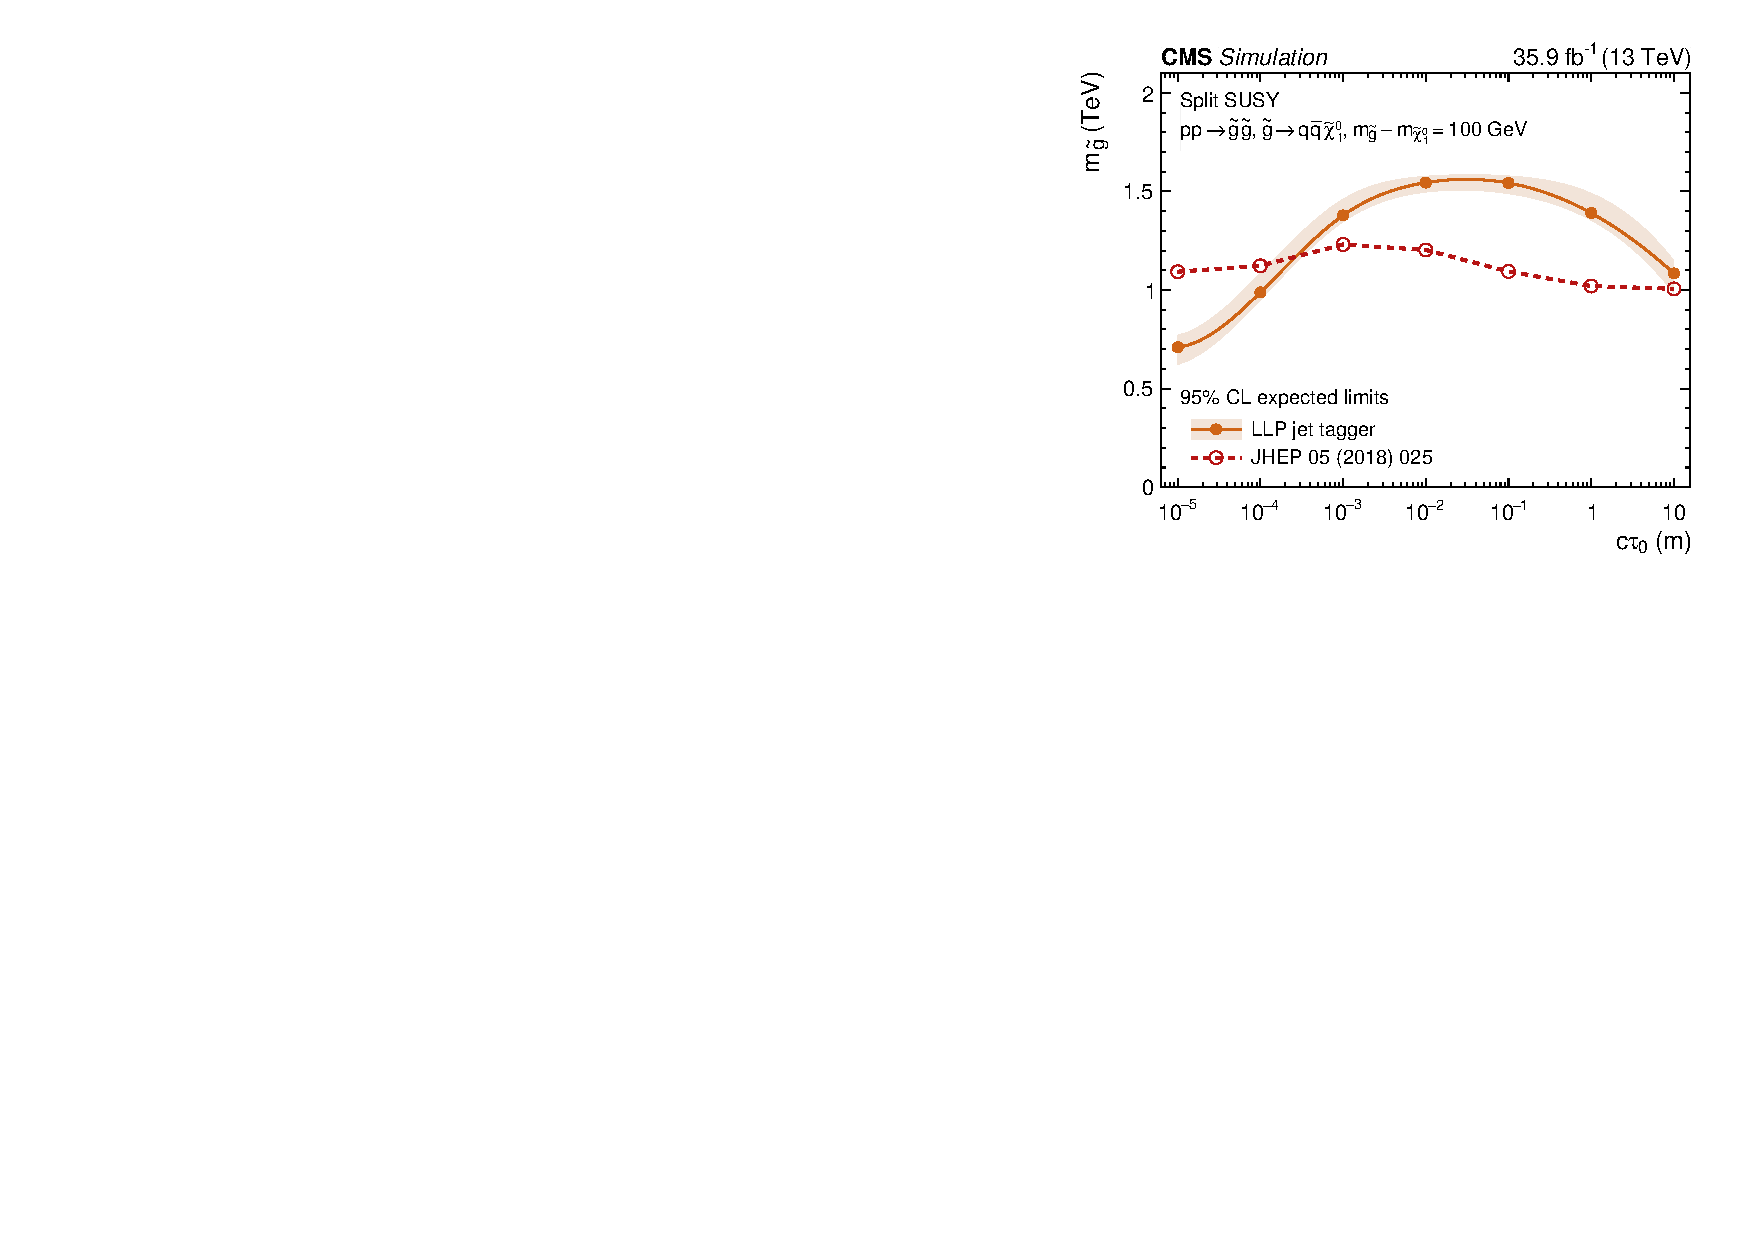
\includegraphics[width=0.48\textwidth]{figs/summaryC.pdf}
\centering
\caption{\label{fig:limits}Expected 95\% CL lower limit on the gluino mass as a function of \ctau for two examples of split SUSY. The figures are taken from Ref.~\cite{CMS-EXO-19-011}.}
\label{fig-4}
\end{figure*}

\section{Summary}
\label{Summary}

In this note, the development and application of a novel algorithm based on a deep neural network is presented to identify displaced jets from the decay of exotic long-lived particles as predicted by various extensions of the standard model of particle physics. To accomplish this task various new techniques are used. A generic definition of a displaced jet is introduced based on generator-truth information that allows to perform supervised learning. In the training, differences between simulation and data are mitigated by applying domain adaptation by backward propagation. The network is parametrised as a function of the lifetime of the long-lived particle, which allows for hypothesis testing over a broad range of lifetimes with just a single network.

The resulting jet tagger is able to reject 99.99\% of light-flavoured jets while retaining 30--80\% of LLP jets for a lifetime range of $1\,\textrm{mm}<\ctau<10\,\textrm{m}$. Lastly, the application of the tagger is demonstrated in a search for split SUSY in which competitive expected limits are determined.

\begin{thebibliography}{}
\bibitem{ml-white-paper} K. Albertsson, et al., J. Phys. Conf. Ser. \textbf{1085} (2018), 022008, \href{http://www.arxiv.org/abs/1807.02876}{arXiv:1807.02876}.
\bibitem{atlas} ATLAS Collaboration, JINST \textbf{3} (2008) S08003, \href{http://dx.doi.org/10.1088/1748-0221/3/08/S08003}{doi:10.1088/1748-0221/3/08/S08003}.
\bibitem{cms}  CMS Collaboration, JINST \textbf{3} (2008) S08004,
\href{http://dx.doi.org/10.1088/1748-0221/3/08/S08004}{doi:10.1088/1748-0221/3/08/S08004}.
\bibitem{batlas} ATLAS Collaboration, Eur. Phys. J. C \textbf{79} (2019) 970, \href{http://dx.doi.org/10.1140/epjc/s10052-019-7450-8}{doi:10.1140/epjc/s10052-019-7450-8}.
\bibitem{bcms} CMS Collaboration, JINST \textbf{13} (2018) P05011,
\href{http://dx.doi.org/10.1088/1748-0221/13/05/P05011}{doi:10.1088/1748-0221/13/05/P05011}.
\bibitem{CMS-EXO-19-011} CMS Collaboration, submitted to MLST, (2019), \href{https://arxiv.org/abs/1912.12238}{arXiv:1912.12238}.
\bibitem{dj} CMS Collaboration, CMS-DP-2018-058, (2018), \href{https://cds.cern.ch/record/2646773}{cds.cern.ch/record/2646773}.
\bibitem{da} Y. Ganin, et al., arXiv e-prints (2014), \href{https://arxiv.org/abs/1409.7495}{arXiv:1409.7495}.
\bibitem{splitsusy} J. L. Hewett et al., JHEP \textbf{09} (2004) 070, \href{http://dx.doi.org/10.1088/1126-6708/2004/09/070}{doi:10.1088/1126-6708/2004/09/070}.
\bibitem{pf} CMS Collaboration, JINST \textbf{12} (2017) P10003, \href{http://dx.doi.org/10.1088/1748-0221/12/10/P10003}{doi:10.1088/1748-0221/12/10/P10003}.
\bibitem{code} M. Komm, et al., Zenodo (2019), \href{http://dx.doi.org/10.5281/zenodo.3571366}{doi:10.5281/zenodo.3571366}.
\bibitem{gmsb} G. F. Giudice, et. al, Phys. Rept. \textbf{322} (1999) 419, \href{http://dx.doi.org/10.1016/S0370-1573(99)00042-3}{doi:10.1016/S0370-1573(99)00042-3}.
\bibitem{rpv} R. Barbier, et. al, Phys. Rept. \textbf{420} (2005) 1, \href{http://dx.doi.org/10.1016/j.physrep.2005.08.006}{doi:10.1016/j.physrep.2005.08.006}.
\bibitem{refsearch} CMS Collaboration, JHEP \textbf{05} (2018) 025, \href{http://dx.doi.org/10.1007/JHEP05(2018)025}{10.1007/JHEP05(2018)025}.
\bibitem{atlasref} ATLAS Collaboration, Phys. Rev. \textbf{D97} (2018) 5, \href{http://dx.doi.org/10.1103/PhysRevD.97.052012}{10.1103/PhysRevD.97.052012}.
\end{thebibliography}

\end{document}
